\documentclass[openany]{book}

\usepackage[margin=1in]{geometry}
\usepackage{amsmath,amsfonts,amsthm, amssymb}
\usepackage{yhmath}
\usepackage{mathrsfs}
\usepackage{mathtools}
\usepackage{xcolor}
\usepackage{graphicx}
\usepackage{comment}
\usepackage{tikz-cd}
\usepackage{quiver}
\renewcommand{\familydefault}{ppl}
\newcommand{\R}{\mathbb{R}}
\newcommand{\E}{\mathbb{E}}
\newcommand{\Z}{\mathbb{Z}}
\newcommand{\CC}{\mathcal{C}}
\newcommand{\F}{\mathbb{F}}
\newcommand{\la}{\langle}
\newcommand{\ra}{\rangle}
\newcommand{\colim}{\text{colim}}
\DeclareMathOperator{\im}{im}
\let\oldemptyset\emptyset
\let\emptyset\varnothing
\newcommand{\tor}{\text{Tor}}
\newcommand{\id}{\text{id}}
\newcommand{\ext}{\text{Ext}}
\newcommand{\ptop}{\text{PTop}}
\newcommand{\pt}{\text{pt}}
\newcommand{\ach}{\text{Ach}}


\usepackage{thmtools,thm-restate}

% Fixing mdframed skip below
% See https://tex.stackexchange.com/a/292090/143086
\usepackage[framemethod=TikZ]{mdframed}
\usepackage{xpatch}
\makeatletter
\xpatchcmd{\endmdframed}
	{\aftergroup\endmdf@trivlist\color@endgroup}
	{\endmdf@trivlist\color@endgroup\@doendpe}
	{}{}
\makeatother

\definecolor{huilightpink}{HTML}{fff2fe}
\definecolor{huidarkpink}{HTML}{d955b7}
\declaretheoremstyle[
	mdframed={
		backgroundcolor=huilightpink,
		linecolor=huidarkpink,
		rightline=false,
		topline=false,
		bottomline=false,
		linewidth=2pt,
		innertopmargin=5pt,
		innerbottommargin=8pt,
		innerleftmargin=8pt,
		leftmargin=-2pt,
		skipbelow=2pt,
		nobreak
	},
	headfont=\normalfont\bfseries\color{huidarkpink}
]{huipinkbox}
\declaretheorem[style=huipinkbox,name=Theorem,within=chapter]{thm}
\declaretheorem[style=huipinkbox,name=Theorem,sibling=thm]{theorem}




\begin{comment}
\definecolor{huilightyellow}{HTML}{fff5d6}
\definecolor{huidarkyellow}{HTML}{fcad03}
\declaretheoremstyle[
	mdframed={
		backgroundcolor=huilightyellow,
		linecolor=huidarkyellow,
		rightline=false,
		topline=false,
		bottomline=false,
		linewidth=2pt,
		innertopmargin=5pt,
		innerbottommargin=8pt,
		innerleftmargin=8pt,
		leftmargin=-2pt,
		skipbelow=2pt,
		nobreak
	},
	headfont=\normalfont\bfseries\color{huidarkyellow}
]{huiyellowbox}
\declaretheorem[style=huiyellowbox,name=Proposition,within=chapter]{prop}
\end{comment}



\definecolor{huilightpurple}{HTML}{faf2ff}
\definecolor{huidarkpurple}{HTML}{912ed9}
\declaretheoremstyle[
	mdframed={
		backgroundcolor=huilightpurple,
		linecolor=huidarkpurple,
		rightline=false,
		topline=false,
		bottomline=false,
		linewidth=2pt,
		innertopmargin=5pt,
		innerbottommargin=8pt,
		innerleftmargin=8pt,
		leftmargin=-2pt,
		skipbelow=2pt,
		nobreak
	},
	headfont=\normalfont\bfseries\color{huidarkpurple}
]{huipurplebox}
\declaretheorem[style=huipurplebox,name=Proposition,within=chapter]{prop}



% \definecolor{huilightpurple}{HTML}{faf2ff}
% \definecolor{huidarkpurple}{HTML}{912ed9}
% \declaretheoremstyle[
% 	mdframed={
% 		backgroundcolor=huilightpurple,
% 		linecolor=huidarkpurple,
% 		rightline=false,
% 		topline=false,
% 		bottomline=false,
% 		linewidth=2pt,
% 		innertopmargin=5pt,
% 		innerbottommargin=8pt,
% 		innerleftmargin=8pt,
% 		leftmargin=-2pt,
% 		skipbelow=2pt,
% 		nobreak
% 	},
% 	headfont=\normalfont\bfseries\color{huidarkpurple}
% ]{huipurplebox}
\declaretheorem[style=huipurplebox,name=Lemma,within=chapter]{lem}


\definecolor{lightpink}{HTML}{f0f6fc}
\definecolor{darkpink}{HTML}{2c72b8}
\declaretheoremstyle[
	mdframed={
		backgroundcolor=lightpink,
		linecolor=darkpink,
		rightline=false,
		topline=false,
		bottomline=false,
		linewidth=2pt,
		innertopmargin=5pt,
		innerbottommargin=8pt,
		innerleftmargin=8pt,
		leftmargin=-2pt,
		skipbelow=2pt,
		nobreak
	},
	headfont=\normalfont\bfseries\color{darkpink}
]{pinkbox}
\declaretheorem[style=pinkbox,name=Definition,within=chapter]{defn}


\definecolor{huilightblue}{HTML}{edf9ff}
\definecolor{huidarkblue}{HTML}{4b79db}
\declaretheoremstyle[
	mdframed={
		backgroundcolor=huilightblue,
		linecolor=huidarkblue,
		rightline=false,
		topline=false,
		bottomline=false,
		linewidth=2pt,
		innertopmargin=5pt,
		innerbottommargin=8pt,
		innerleftmargin=8pt,
		leftmargin=-2pt,
		skipbelow=2pt,
		nobreak
	},
	headfont=\normalfont\bfseries\color{huidarkblue}
]{huiblueblox}
\declaretheorem[style=huiblueblox,name=Example,within=chapter]{example}



% \definecolor{huilightblue}{HTML}{edf9ff}
% \definecolor{huidarkblue}{HTML}{4b79db}
% \declaretheoremstyle[
% 	mdframed={
% 		backgroundcolor=huilightblue,
% 		linecolor=huidarkblue,
% 		rightline=false,
% 		topline=false,
% 		bottomline=false,
% 		linewidth=2pt,
% 		innertopmargin=5pt,
% 		innerbottommargin=8pt,
% 		innerleftmargin=8pt,
% 		leftmargin=-2pt,
% 		skipbelow=2pt,
% 		nobreak
% 	},
% 	headfont=\normalfont\bfseries\color{huidarkblue}
% ]{huiblueblox}
% \declaretheorem[style=huiblueblox,name=Example,within=chapter]{example}

% \declaretheoremstyle[
% 	mdframed={
% 		backgroundcolor=huilightblue,
% 		linecolor=huidarkblue,
% 		rightline=false,
% 		topline=false,
% 		bottomline=false,
% 		linewidth=2pt,
% 		innertopmargin=5pt,
% 		innerbottommargin=8pt,
% 		innerleftmargin=8pt,
% 		leftmargin=-2pt,
% 		skipbelow=2pt,
% 		nobreak
% 	},
% 	headfont=\normalfont\bfseries\color{huidarkblue}
% ]{huiblueblox}
\declaretheorem[style=huiblueblox,name=Problem,within=chapter]{prob}



% \declaretheoremstyle[
% 	mdframed={
% 		backgroundcolor=huilightblue,
% 		linecolor=huidarkblue,
% 		rightline=false,
% 		topline=false,
% 		bottomline=false,
% 		linewidth=2pt,
% 		innertopmargin=5pt,
% 		innerbottommargin=8pt,
% 		innerleftmargin=8pt,
% 		leftmargin=-2pt,
% 		skipbelow=2pt,
% 		nobreak
% 	},
% 	headfont=\normalfont\bfseries\color{huidarkblue}
% ]{huiblueblox}
\declaretheorem[style=huiblueblox,name=Exercise,within=chapter]{exer}
\declaretheorem[style=huipinkbox, name=Corollary, within=chapter]{cor}





















\newcommand{\nirwarnsymbol}{%
	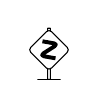
\begin{tikzpicture}[baseline=(x.base)]
		\draw[rounded corners=.01em] (-.05em,-1.07em)rectangle(.05em,.78em);
		\draw[fill=white,rounded corners=1.3] (0,.75em)--(.75em,0)--(0,-.75em)--(-.75em,0)--cycle;
		\draw[line width=0.2mm, line cap=round](-.4em,-1.07em)--(.4em,-1.07em);
		\node(x) at (0,0em) {};
		% Thank you https://tex.stackexchange.com/a/262510
		\draw[
			line cap=but,
			line join=round,
			x=.5em,
			line width=0.5mm,
			y=1*(height("Z")-\pgflinewidth)*(1-sin(10)),
			rotate=-10,
			rounded corners=1.5pt,
		](-0.57, 0.57) -- (0.57, 0.57) -- (-0.57, -0.57) -- (0.57, -0.57);
	\end{tikzpicture}%
}

%%%%%%%%%%%%%%%%%%%%%%%%%%%%%%%%%%%%%%%%%%%% MARGINS
\usepackage{marginnote}
% Thank you https://tex.stackexchange.com/a/472882
% Makes marginnotes always appear on the left, apparently
%
\makeatletter
\long\def\@mn@@@marginnote[#1]#2[#3]{%
	\begingroup
		\ifmmode\mn@strut\let\@tempa\mn@vadjust\else
			\if@inlabel\leavevmode\fi
			\ifhmode\mn@strut\let\@tempa\mn@vadjust\else\let\@tempa\mn@vlap\fi
		\fi
		\@tempa{%
			\vbox to\z@{%
				\vss
				\@mn@margintest
				\if@reversemargin\if@tempswa
						\@tempswafalse
					\else
						\@tempswatrue
				\fi\fi

					\llap{%
						\vbox to\z@{\kern\marginnotevadjust\kern #3
							\vbox to\z@{%
								\hsize\marginparwidth
								\linewidth\hsize
								\kern-\parskip
								%\mn@parboxrestore
								\marginfont\raggedleftmarginnote\strut\hspace{\z@}%
								\ignorespaces#1\endgraf
								\vss
							}%
							\vss
						}%
						\if@mn@verbose
							\PackageInfo{marginnote}{xpos seems to be \@mn@currxpos}%
						\fi
						\begingroup
							\ifx\@mn@currxpos\relax\else\ifx\@mn@currpos\@empty\else
									\kern\@mn@currxpos
							\fi\fi
							\ifx\@mn@currpage\relax
								\let\@mn@currpage\@ne
							\fi
							\if@twoside\ifodd\@mn@currpage\relax
									\kern-\oddsidemargin
								\else
									\kern-\evensidemargin
								\fi
							\else
								\kern-\oddsidemargin
							\fi
							\kern-1in
						\endgroup
						\kern\marginparsep
					}%
			}%
		}%
	\endgroup
}
\makeatother
%
% Mostly for todonotes
\renewcommand{\marginpar}{\marginnote}
%%%%%%%%%%%%%%%%%%%%%%%%%%%%%%%%%%%%%%%%%%%% /MARGINS

\definecolor{nirlightred}{RGB}{250, 220, 220}
\definecolor{nirdarkred}{HTML}{f40000}
\declaretheoremstyle[
	mdframed={
		backgroundcolor=nirlightred,
		linecolor=nirdarkred,
		rightline=false,
		topline=false,
		bottomline=false,
		linewidth=2pt,
		innertopmargin=5pt,
		innerbottommargin=8pt,
		innerleftmargin=8pt,
		leftmargin=-2pt,
		skipbelow=2pt,
		nobreak
	},
	headfont=\normalfont\bfseries\color{nirdarkred}
]{nirredbox}

% \makeatletter
% \declaretheorem[
% 	style=nirredbox,
% 	name=Warning,
% 	sibling=thm,
% 	% without \leavevmode, the first item in a list gets misformatted
% 	postheadhook={\leavevmode\marginnote{\nirwarnsymbol}[-3pt]%
% 	\ifthmt@thisistheone% restatable makes alignment weird
% 		\hspace{-2.2pt}%
% 	\fi}
% ]{warn}
% \makeatother

\newcommand{\nirideasymbol}{%
	
\begin{tikzpicture}[baseline=(x.base)]
		\draw[rounded corners=.01em] (-.05em,-1.07em)rectangle(.05em,.78em);
		\draw[fill=white,rounded corners=1.3] (0,.75em)--(.75em,0)--(0,-.75em)--(-.75em,0)--cycle;
		\draw[line width=0.2mm, line cap=round](-.4em,-1.07em)--(.4em,-1.07em);
		\node(x) at (0,0em) {};
		\node at (0,0em) {{\textbf{!}}};
	\end{tikzpicture}%
}
\renewcommand{\nirwarnsymbol}{%
	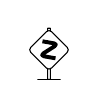
\begin{tikzpicture}[baseline=(x.base)]
		\draw[rounded corners=.01em] (-.05em,-1.07em)rectangle(.05em,.78em);
		\draw[fill=white,rounded corners=1.3] (0,.75em)--(.75em,0)--(0,-.75em)--(-.75em,0)--cycle;
		\draw[line width=0.2mm, line cap=round](-.4em,-1.07em)--(.4em,-1.07em);
		\node(x) at (0,0em) {};
		% Thank you https://tex.stackexchange.com/a/262510
		\draw[
			line cap=but,
			line join=round,
			x=.5em,
			line width=0.5mm,
			y=1*(height("Z")-\pgflinewidth)*(1-sin(10)),
			rotate=-10,
			rounded corners=1.5pt,
		](-0.57, 0.57) -- (0.57, 0.57) -- (-0.57, -0.57) -- (0.57, -0.57);
	\end{tikzpicture}%
}
\makeatletter
\declaretheorem[
	style=nirredbox,
	name=Idea,
	sibling=thm,
	% without \leavevmode, the first item in a list gets misformatted
	postheadhook={\leavevmode\marginnote{\nirideasymbol}[-3pt]%
	\ifthmt@thisistheone% restatable makes alignment weird
		\hspace{-2.2pt}%
	\fi}
]{idea}

\declaretheorem[
	style=nirredbox,
	name=Warning,
	sibling=thm,
	% without \leavevmode, the first item in a list gets misformatted
	postheadhook={\leavevmode\marginnote{\nirwarnsymbol}[-3pt]%
	\ifthmt@thisistheone% restatable makes alignment weird
		\hspace{-2.2pt}%
	\fi}
]{warn}
\makeatother

\title{Fourier Analysis}

\date{\today}
\author{Hui Sun}

\begin{document}

\maketitle

\tableofcontents



\newpage

\chapter{The Gensis of Fourier Analysis}

In this chapter, we will motivate the study of Fourier analysis: explaining the roles of $\cos t, \sin t, e^{it}$, learning about the motion of vibrating string, finding its solution, and finally, studying heat diffusion. (The aim of this chapter is to motivate more rigorous study of Fourier analysis in later chapters, feel free to skip to Chapter 2.)

\section{The vibrating string}






\chapter{Basic properties of Fourier series}

In this chapter, we define Fourier series, briefly discuss the question of pointwise convergence of Fourier series.

\section{Definition of Fourier series}
We ask the readers to review or read the concepts of integrable functions on their own. We begin with functions on the circle: a point on the unit circle always takes the form $e^{i\theta}$, where $\theta$ is unique up to multiples of $2\pi$. Therefore a function on the circle can be written as 
\begin{equation*}
    f(\theta)=F(e^{i\theta})
\end{equation*}
Notice that $f(\theta)=f(\theta+2\pi)$, and on ther other hand, if $f$ defined on $\R$ is periodic with period $2\pi$, then we also have $f(x)=f(x+2\pi)$, for any $x\in\R$. This establishes that every periodic $f$ on $\R$ with period $2\pi$ can be identified with a function defined on the circle $\mathbb{T}$.

We now define Fourier series.
\begin{defn}[Fourier series]
    Let $f$ be an integrable function defined on $[0,2\pi]$, then its nth Fourier coefficient is 
\begin{equation*}
    \hat{f}(n)=\frac{1}{2\pi}\int_0^{2\pi}f(x)e^{-inx}dx, \quad n\in\mathbb{Z}
\end{equation*}
The Fourier series of $f$ is given formally by 
\begin{equation*}
    f(x)\sim \sum_{n=-\infty}^{\infty}\hat{f}(n)e^{inx}
\end{equation*}
    where $\sim$ notation denotes the Fourier series.
\end{defn}
The book defines Fourier series for $f$ defined on an interval $[0,L]$, which we will omit here. We will now calculate the Fourier series of some functions now.
\begin{example}
    \begin{enumerate}
        \item Let $f(\theta)=\theta, -\pi\leq\theta\leq\pi$, then 
        \begin{equation*}
            f(\theta)\sim\sum_{n\neq 0}\frac{(-1)^{n+1}}{in}e^{in\theta}
        \end{equation*}
        \item Let $f(\theta)=(\pi-\theta)^2/4$, for $0\leq\theta\leq 2\pi$, then we find 
        \begin{equation*}
            f(\theta)\sim\frac{\pi^2}{12}+\sum_{n=1}^\infty\frac{\cos n\theta}{n^2}
        \end{equation*}
        \item Let $f(\theta)=\frac{\pi}{\sin\pi\alpha}e^{i(\pi-\theta)\alpha}$ defined on $[0,2\pi]$, when $\alpha$ is not an integer, and the Fourier series is given by 
        \begin{equation*}
            f(\theta)\sim\sum_{n=-\infty}^{\infty}\frac{e^{in\theta}}{n+\alpha}
        \end{equation*}
    \end{enumerate}
\end{example}
\begin{proof}
    The book computes 1, and here we will do 2 and 3. For $f(\theta)=(\pi-\theta)^2/4$, when $n=0$, we have
    \begin{align*}
        \hat{f}(0)&=\frac{1}{8\pi}\int_0^{2\pi}(\pi-\theta)^2d\theta\\
        &=\frac{\pi^2}{12}
    \end{align*}
    When $n\neq 0$, we have
    \begin{align*}
        8\pi\hat{f}(n)&=\int_0^{2\pi}(\pi-\theta)^2e^{-in\theta}\\
        &=\left[\frac{(\pi-\theta)^2}{-in}e^{-in\theta}\right]_{0}^{2\pi}-2\int_0^{2\pi}(\pi-\theta)\frac{e^{-in\theta}}{-in}d\theta\\
        &=-2\left[(\pi-\theta)\frac{e^{-in\theta}}{n^2}\right]_0^{2\pi}-2\int_0^{2\pi}\frac{e^{-in\theta}}{n^2}d\theta\\
        &=\frac{4\pi}{n^2}
    \end{align*}
    Hence the Fourier series is given by 
    \begin{align*}
        f(\theta)&\sim \sum_{n=-\infty}^\infty \hat{f}(n)e^{in\theta}\\
        &=\frac{\pi^2}{12}+\sum_{n\neq 0}\frac{1}{2n^2}e^{in\theta}\\
        &=\frac{\pi^2}{12}+\sum_{n\neq 0}\frac{1}{2n^2}(\cos n\theta+i\sin n\theta)\\
        &=\frac{\pi^2}{12}+\sum_{n=1}^\infty \frac{1}{2n^2}\left(\cos n\theta+\cos(-n\theta)\right)+\frac{1}{2n^2}\left(i\sin n\theta+i\sin -n\theta\right)\\
        &=\frac{\pi^2}{12}+\sum_{n=1}^\infty\frac{\cos n\theta}{n^2}
    \end{align*}
    as desired.

    \noindent
    3. For $f(\theta)=\frac{\pi}{\sin\pi\alpha}e^{i(\pi-\theta)\alpha}$ defined on $[0,2\pi]$, when $\alpha$ is not an integer, we compute
    \begin{align*}
        \left(\frac{1}{2\pi}\frac{\pi}{\sin\pi\alpha}e^{i\pi\alpha}\right)^{-1}\hat{f}(n)&=\int_0^{2\pi}e^{-i\theta\alpha}e^{-in\theta}d\theta\\
        &=\int_0^{2\pi}e^{-i(n+\alpha)\theta}d\theta\\
        &=\left[\frac{e^{-i(n+\alpha)\theta}}{-in(n+\alpha)}\right]_{\theta=0}^{2\pi}\\
        &=\frac{1-e^{-2\pi i\alpha}}{i(n+\alpha)}
    \end{align*}
    This gives that 
    \begin{align*}
        \hat{f}(n)&=\frac{1-e^{-2\pi i\alpha}}{2i(n+\alpha)}\frac{e^{i\pi\alpha}}{\sin\pi\alpha}\\
        &=\frac{1-e^{-2\pi i\alpha}}{2i(n+\alpha)}\frac{e^{i\pi\alpha}\cdot 2i}{e^{i\pi\alpha}-e^{-i\pi\alpha}}\\
        &=\frac{1}{n+\alpha}
    \end{align*}
    This implies that 
    \begin{equation*}
        f(\theta)\sim\sum_{n=-\infty}^\infty \frac{e^{in\theta}}{n+\alpha}
    \end{equation*}
\end{proof}
Next we introduce two special trigonometric polynomials and series that we will discuss later: the $N$th \textbf{ Dirichlet kernel} $D_N$ is defined as
\begin{equation*}
    D_N(x)=\sum_{n=-N}^Ne^{inx}
\end{equation*} 
and the \textbf{Poisson kernel} $P_r(\theta)$ is the series for $\theta\in [-\pi,\pi]$, and for $0\leq r<1$, 
\begin{equation*}
    P_r(\theta)=\sum_{n=-\infty}^\infty r^{|n|}e^{in\theta}
\end{equation*}
We notice that $P_r(\theta)$ converges absolutely, hence we can compute 
\begin{align*}
    \hat{P}_r(m)&=\frac{1}{2\pi}\int_{-\pi}^{\pi}\sum_{n=-\infty}^\infty r^{|n|}e^{i(n-m)\theta}d\theta\\
    &=\frac{1}{2\pi}\sum_{n=-\infty}^\infty\int_{-\pi}^\pi r^{|n|}e^{i(n-m)\theta}d\theta\\
    &=r^{|m|}
\end{align*}
this means the $n$th Fourier coefficient of the Poisson kernel is $r^{|n|}$. Again, we will talk about these kernels in a little bit.

Now we introduced the Fourier series a function $f$, 
\begin{equation*}
    f(\theta)\sim \sum_{n=-\infty}^\infty \hat{f}(n)e^{in\theta}
\end{equation*}
we ask the question whether the Fourier series converges to $f$ pointwise. 
\begin{prob}\label{2.1}
    What assumptions of $f$ are needed, such that 
    \begin{equation}
        \lim_{N\to\infty}\sum_{n=-N}^N\hat{f}(n)e^{in\theta}=f(\theta)
    \end{equation}
    for all $\theta\in [-\pi,\pi]$.
\end{prob}
We will now start answering this question: we will begin by showing that functions $f$ that are twice continuously differentiable over $[-\pi,\pi]$ have Fourier series converges pointwise to $f$. We first establish some properties of Fourier series leading to this result.

\begin{thm}[Uniqueness of Fourier series]
    Let $f$ be an integrable function on the circle, where $\hat{f}(n)=0$ for all $n\in\mathbb{Z}$. Then $f(x)=0$ for all points of continuity $x$. 
\end{thm}
The proof is omitted here and the reader can refer to the book, the idea is that assume $f(x)\neq 0$, then it constructs a family of trigonometric polynomials that peaks at $x$, therefore multiplying them together contradicts the fact that $\hat{f}(n)=0$ for all $n$. An immediate corollary is as follows:
\begin{cor}
    Let $f,g$ be two continuous functions on the circle, if $\hat{f}(n)=\hat{g}(n)$ for all $n\in\mathbb{Z}$, then 
    \begin{equation*}
        f=g
    \end{equation*}
\end{cor}
This corollary allows us to prove the following result, which is a partial answer to the problem in \ref{2.1}
\begin{prop}
    Let $f$ be a continuous function on the cirlce, if $\sum|\hat{f}(n)|<\infty$, then 
    \begin{equation*}
        \lim_{N\to\infty}S_N(f)(\theta)=f(\theta) \quad \text{ uniformly in } \theta 
    \end{equation*}
    where $S_N(f)(\theta)=\sum_{n=-N}^N\hat{f}(n)e^{in\theta}$.
\end{prop}
\begin{proof}
    (The idea is to show that $S_N(f)(\theta)$ converges to $\sum_{n=-\infty}^\infty\hat{f}(n)e^{in\theta}:=g(\theta)$ absolutely and uniformly. This would imply that $g$ is continuous, then we find $\hat{g}(n)=\hat{f}(n)$, and by the above corollary, $g=f$, hence $S_N(f)$ converges to $f$.) Because $\sum_n|\hat{f}(n)|<\infty$, for any $\varepsilon>0$, there exists $m$ such that for every $\theta$, we have 
    \begin{equation*}
        \left|\sum_{|n|\geq m}\hat{f}(n)\right|\leq \sum_{|n|\geq m}|\hat{f}(n)|<\varepsilon
    \end{equation*}
    denote $g(\theta)=\sum_{n=-\infty}^\infty\hat{f}(n)e^{in\theta}$, this implies that 
    \begin{equation*}
        \lim_{N\to\infty}S_N(f)(\theta)=g(\theta)
    \end{equation*}
    absolutely and uniformly. Since $S_N(f)$ is a sequence of continuous functions, this shows that $g$ is also continuous. Now 
    \begin{align*}
        \hat{g}(n)&=\frac{1}{2\pi}\int_{0}^{2\pi}\sum_{k=-\infty}^\infty\hat{f}(k)e^{ik\theta}e^{-in\theta}d\theta\\
        &=\sum_{k=-\infty}^\infty\frac{1}{2\pi}\int_{0}^{2\pi}\hat{f}(k)e^{i(k-n)\theta}d\theta\\
        &=\hat{f}(n)
    \end{align*}
    Hence by the previous corollary, we see that $f=g$, i.e., 
    \begin{equation*}
        \lim_{N\to\infty}S_N(f)(\theta)=f(\theta)
    \end{equation*}
\end{proof}
Using this criterion of absolute convergence of Fourier coefficients, we have the following result.
\begin{cor}[twice continuously differentiable]
    Let $f$ be a twice continuously differentiable function on the circle, then 
    \begin{equation*}
        \hat{f}(n)=O\left(1/|n|^2\right) \text{ as } |n|\to\infty
    \end{equation*}
    Moreover, the Fourier series $f$ converges to $f$ absolutely and uniformly in $\theta$.
\end{cor}
\begin{proof}
    If $\hat{f}(n)=O\left(1/|n|^2\right)$ as $|n|\to\infty$, then the Fourier series of $f$ converges absolutely. And by the previous corollary, it converges to $f$ uniformly in $\theta$. Therefore it suffices to show $\hat{f}(n)=O\left(1/|n|^2\right)$, as $|n|\to\infty$, so we can assume $n\neq 0$,
    \begin{align*}
        2\pi\hat{f}(n)&=\int_0^{2\pi}f(\theta)e^{-in\theta}d\theta\\
        &=\left[f(\theta)\cdot\frac{-e^{-in\theta}}{in}\right]_0^{2\pi}+\frac{1}{in}\int_0^{2\pi}f'(\theta)e^{-in\theta}d\theta\\
        &=\frac{1}{in}\left[f'(\theta)\cdot\frac{-e^{-in\theta}}{in}\right]_0^{2\pi}-\frac{1}{n^2}\int_0^{2\pi}f''(\theta)e^{-in\theta}d\theta
    \end{align*}
    This implies that 
    \begin{equation*}
        \left|\hat{f}(n)\right|\leq \frac{1}{2\pi n^2}\int_0^{2\pi}|f''(\theta)|d\theta\leq C/n^2
    \end{equation*}
    We thus have 
    \begin{equation*}
        \hat{f}(n)=O\left(1/|n|^2\right)
    \end{equation*}
    as desired.
\end{proof}
In fact, functions that are $k$ times continuously differentiable, i.e., $C^k$ where $k\geq 2$, have Fourier coefficients behave as 
\begin{equation*}
    \hat{f}(n)=O\left(1/|n|^k\right)
\end{equation*}
And naturally, $C^k$ functions have Fourier series converge to them uniformly. This highlights a key property of Fourier series: the smoother the function, the better the Fourier series convergence.

Next we will talk about convolutions and how it relates to the Fourier series.
\begin{defn}[convolution]
    Let $f,g$ be two functions defined on the circle, then their \textbf{convolution} is defined as 
    \begin{equation*}
        f\ast g(x)=\frac{1}{2\pi}\int_{-\pi}^\pi f(y)g(x-y)dy
    \end{equation*}
\end{defn}
One can interpret convolution as ``weighted average'': if $g=1$, then $f\ast g\equiv\int_{-\pi}^{\pi}f(y)dy$, i.e., the average value of $f$. We will see in a little bit that if $g$ takes the form of an ``approximation to identity'', then $f\ast g(x)$ will recover $f(x)$. We will record without proof some of the properties of convolution.
\begin{prop}[Properties of convolutions]
    Suppose $f,g,h$ are functions are the circle, then 
    \begin{enumerate}
        \item $f\ast(g+h)=f\ast g+f\ast h$
        \item $(cf)\ast g=c(f\ast g)=f\ast (cg) \text{ for any } c\in\mathbb{C}$
        \item $f\ast g=g\ast f$
        \item $(f\ast g)\ast h=f\ast(g\ast h)$
        \item Given $f,g$ are integrable, $f\ast g$ is continuous.
        \item Fourier transform of the convolution is the product of the Fourier transforms:
        \begin{equation*}
            \widehat{f\ast g}(n)=\hat{f}\hat{g}(n)
        \end{equation*}
    \end{enumerate}
\end{prop}
We will highlight 5, which states that convolution of two integrable functions is continuous, this means convolution improves the smoothness of the functions given. We will often use 6, but it is not a hard identity to check. The reason we introduce convolutions is as follows:
\begin{align*}
    S_N(f)(x)&=\sum_{n=-N}^N\hat{f}(n)e^{inx}\\
    &=\frac{1}{2\pi}\sum_{n=-N}^N\int_{-\pi}^\pi f(y)e^{in(x-y)}dy\\
    &=\frac{1}{2\pi}\int_{-\pi}^\pi f(y)\left(\sum_{n=-N}^Ne^{in(x-y)}\right)dy\\
    &=f\ast D_N(x)
\end{align*}
where $D_N$ is the Dirichlet kernel
\begin{equation*}
    D_N(x)=\sum_{n=-N}^N e^{inx}
\end{equation*}
Therefore the question of whether $S_N(f)(x)$ converges to $f(x)$ becomes the question under what conditions does 
\begin{equation*}
    f\ast D_N(x)\to f(x)
\end{equation*}
as $N\to\infty$. For this, we introduce approximation to identity, which the textbook titles the section as ``good kernels.''

We can examine $f\ast K_N$ for any family of kernels $K_n$ and ask the question whether $f\ast K_N(x)\to f(x)$. To answer this question, we define approximation to identity.
\begin{defn}[approximation to identity]
    A family of kernels $\{K_n\}$ is said to be a family of good kernels if it satisfies:
    \begin{enumerate}
        \item For all $n\geq 1$, 
        \begin{equation*}
            \frac{1}{2\pi}\int_{-\pi}^\pi K_n(x)dx=1
        \end{equation*}
        \item There exists $M>0$ such that for all $n$, 
        \begin{equation*}
            \int_{-\pi}^\pi|K_n(x)|dx\leq M
        \end{equation*}
        \item For every $\delta>0$, 
        \begin{equation*}
            \int_{\delta\leq|x|\leq\pi}|K_n(x)|dx\to 0 \text{ as } n\to\infty
        \end{equation*}
    \end{enumerate}
\end{defn}
In fact, there is usually a more standard way of constructing approximation to identity: let $\phi$ be an integrable function on the circle and $\int\phi=1$, and define $\phi_t(x)=t^{-1}\phi(x/t)$, and as $t\to 0$, if $g$ is continuous, then
\begin{equation*}
    \lim_{t\to 0}\phi_t\ast g(x)=g(x)
\end{equation*}
The reason why we introduce them is precisely the following:
\begin{thm}
    Let $\{K_n\}_{n=1}^\infty$ be a family of good kernels, and $f$ is an integrable function on the circle. Then if $f$ is continuous at $x$. 
    \begin{equation*}
        \lim_{n\to\infty}(f\ast K_n)(x)=f(x)
    \end{equation*}
    That is, if $f$ is continuous, then 
    \begin{equation*}
        \lim_{n\to\infty}(f\ast K_n)(x)=f(x) \text{ uniformly in } x \text{ as } n\to\infty
    \end{equation*}
\end{thm}
\begin{proof}
    This proof is quite important. Suppose $f$ is continuous at $x$, then for any $\varepsilon>0$, there exists $\delta$ such that when $|y|<\delta$, then $|f(x-y)-f(x)|<\varepsilon$. Fix some $\varepsilon>0$, we choose $\delta>0$ such that $|f(x-y)-f(x)|<\varepsilon$, we also note that there exists $B$ such that $|f(x)|\leq B$ for all $x$. Hence we have
    \begin{align*}
        (f\ast K_n)(x)-f(x)&=\frac{1}{2\pi}\int_{-\pi}^\pi K_n(y)f(x-y)dy-f(x)\\
        &=\frac{1}{2\pi}\int_{-\pi}^\pi K_n(y)\left[f(x-y)-f(x)\right]dy\\
        &=\frac{1}{2\pi}\int_{|y|\leq \delta}K_n(y)\left[f(x-y)-f(x)\right]dy+\frac{1}{2\pi}\int_{\delta\leq|y|\leq\pi}K_n(y)\left[f(x-y)-f(x)\right]dy\\
        &\leq\frac{\varepsilon}{2\pi}\int_{|y|\leq\delta}|K_n(y)|dy+\frac{2B}{2\pi}\int_{\delta\leq|y|\leq\pi}|K_n(y)|dy\\
        &\leq\frac{\varepsilon M}{2\pi}+\frac{\varepsilon B}{\pi}
    \end{align*}
    by letting $n\to\infty$. Hence letting $\varepsilon\to 0$, we see that 
    \begin{equation*}
        \lim_{n\to\infty} f\ast K_n(x)=f(x)
    \end{equation*}
    if $f$ is continuous at $x$.
\end{proof}
Recall that the (partial sum of )Fourier series of $f$ can be expressed as 
\begin{equation*}
    S_Nf(x)=f\ast D_N(x)
\end{equation*}
\begin{warn}
    Hence it'd be nice if the Dirichlet kernel was a good kernel because that would imply that continuous functions have convergent Fourier series! This is not the case: Dirichlet kernel is not a good kernel. More upsettingly, there exists continuous functions whose Fourier series diverge everywhere!
\end{warn}

\section{Cesaro and Abel summability: applications to Fourier series}
In this section, we will introduce convergence in a different sense: continuous functions $f$ have Fourier series that are Cesaro summable and Abel summable!

\begin{defn}[Cesaro sum]
    Suppose we have a series $\sum_{k}c_k$, and we define its $n$th partial sum as 
    \begin{equation*}
        s_n=\sum_{k=0}^n c_k
    \end{equation*}
    then we define its $N$th Cesaro sum as 
    \begin{equation*}
        \sigma_N=\frac{s_0+s_1+\dots+s_{N-1}}{N}
    \end{equation*}
    If $\sigma_N$ converges to $\sigma$ as $N\to\infty$, then $\sum_kc_k$ is said to be \textbf{Cesaro summable} to $\sigma$. 
\end{defn}
We need to check this definition makes sense: if $\sum_kc_k$ converges to $s$ in the usual sense, then $\sum_kc_k$ is also Cesaro summable to $s$. (We will show this in an exercise).

\noindent
Just like the Fourier series can be written in terms of a kernel, the Cesaro sum of Fourier series can also be written as a kernel: let $\sigma_Nf$ denote the $N$th Cesaro sum of Fourier series, we have
\begin{align*}
    \sigma_Nf(x)&=\frac{S_0f(x)+\dots+S_{N-1}f(x)}{N}\\
    &=f\ast\frac{D_0(x)+\dots+D_{N-1}(x)}{N}
\end{align*}
since $S_nf=f\ast D_n$. Let 
\begin{equation*}
    F_N(x)=\frac{D_0(x)+\dots+D_{N-1}(x)}{N}
\end{equation*}
this is known as the \textbf{Fejer kernel}. One can check that the Fejer kernel is a good kernel, hence we have the following corollary.
\begin{cor}
    We have the following:
    \begin{enumerate}
        \item  If $f$ is integrable on the circle and $f$ is continuous at $x$, then its Fourier series is Cesaro summable to $f$ at $x$.
        \item If $f$ is integrable on the circle and continuous at $x$, if $\hat{f}(n)=0$ for all $n$, then $f(x)=0$.
        \item If $f$ on the circle is continuous, then the Fourier series is uniformly Cesaro summable to $f$.
    \end{enumerate}
\end{cor}
We will play more with this concept in the exercises. Next we introduce another way to convergence.

\begin{defn}[Abel sum]
    A series of $\sum_kc_k$ s Abel summable to $s$ if the series 
    \begin{equation*}
        A(r)=\sum_{k=0}^\infty c_kr^k
    \end{equation*}
    converges for every $0\leq r<1$, and 
    \begin{equation*}
        \lim_{r\to 1}A_r(s)=1
    \end{equation*}
    where $A(r)$ is called the \textbf{Abel sum}. 
\end{defn}
The next proposition states that Cesaro implies Abel, but the arrow is not reversed.
\begin{prop}\label{prop23}
    If a series $\sum_kc_k$ is Cesaro summable, then it is Abel summable. However, Cesaro summable does not imply Abel summable.
\end{prop}
\begin{proof}
    The proof that Cesaro implies Abel summable be found in the exercises. Here we will simply give an example of an Abel summable series that is not Cesaro summable:
    \begin{equation*}
        \sum_{n=1}^\infty (-1)^{n-1}n
    \end{equation*}
    We claim this series is Abel summable. For $0\leq r<1$, we first note that  
    \begin{equation*}
        \sum_{n=1}^\infty nr^{n-1}=\frac{1}{(1-r)^2}
    \end{equation*}
    Hence we have 
    \begin{equation*}
        \sum_{n=1}^\infty nr^n=\frac{r}{(1-r)^2}\Rightarrow \sum_{n=1}^\infty (-1)^n nr^n=\frac{-r}{(1+r)^2}\Rightarrow \sum_{n=1}^\infty (-1)^{n-1}nr^n=\frac{r}{(1+r)^2}
    \end{equation*}
    and letting $r\to 1$, we see the series is Abel summable to $\frac{1}{4}$. However, it is not Cesaro summable.

    We know that if a series is Cesaro summable, then 
    \begin{equation*}
        \sigma_n=\sum_{k=1}^n\frac{c_k}{n}\to s
    \end{equation*}
    as $n\to\infty$, this implies that $\frac{c_n}{n}\to 0$ as $n\to\infty$, but clearly in this case $c_n/n=(-1)^{n-1}\neq 0$, i.e., not Cesaro summable.
\end{proof}
Then similarly, we define the Abel means of Fourier series:
\begin{equation*}
    A_rf(\theta)=\sum_{n=-\infty}^\infty r^{|n|}\hat{f}(n)e^{in\theta}
\end{equation*}
if we define the \textbf{Poisson kernel} to be 
\begin{equation*}
    P_r(\theta)=\sum_{n=-\infty}^\infty r^{|n|}e^{in\theta}
\end{equation*}
then we see that 
\begin{equation*}
    A_rf(\theta)=(f\ast P_r)(\theta)
\end{equation*}
Just like above, one can show that the Poisson kernel is a good kernel and conclude Proposition \ref{prop23} applies to Abel summability.











\end{document}